\documentclass[landscape,footrule]{foils}
\usepackage[lecture-serie]{foiltex-extra}
\usepackage{crysymb}
\usepackage{graphics}
\usepackage[pdftex]{graphicx} 




\newcommand{\lecture}{Introduction}
\newcommand{\lserie}{LTAT.02.004 Machine Learning II}
\newcommand{\ldate}{12 February, 2013}
\newcommand{\lauthor}{Sven Laur}
\newcommand{\linst}{University of Tartu}
\graphicspath{{./illustrations/}}
\MyLogo{\lserie,\  Association rules and decision trees, \ldate}


\newcommand{\leqm}{\ \leq_m}


\newcommand{\bigvskip}{\vskip 2em}
\newcommand{\lastline}{\vspace*{-2ex}}
\newcommand{\spreadappart}{\vspace*{\fill}}

\DeclareMathOperator{\supp}{supp}
\DeclareMathOperator{\conf}{conf}
\DeclareMathOperator{\precision}{precision}
\DeclareMathOperator{\recall}{recall}


\begin{document}
\titlefoil


\foilhead[-1cm]{Four basic tasks in machine learning}
\enlargethispage{3cm}
\begin{tabbing}
 \hspace*{2cm}\=\hspace*{10cm}\=\kill
   \>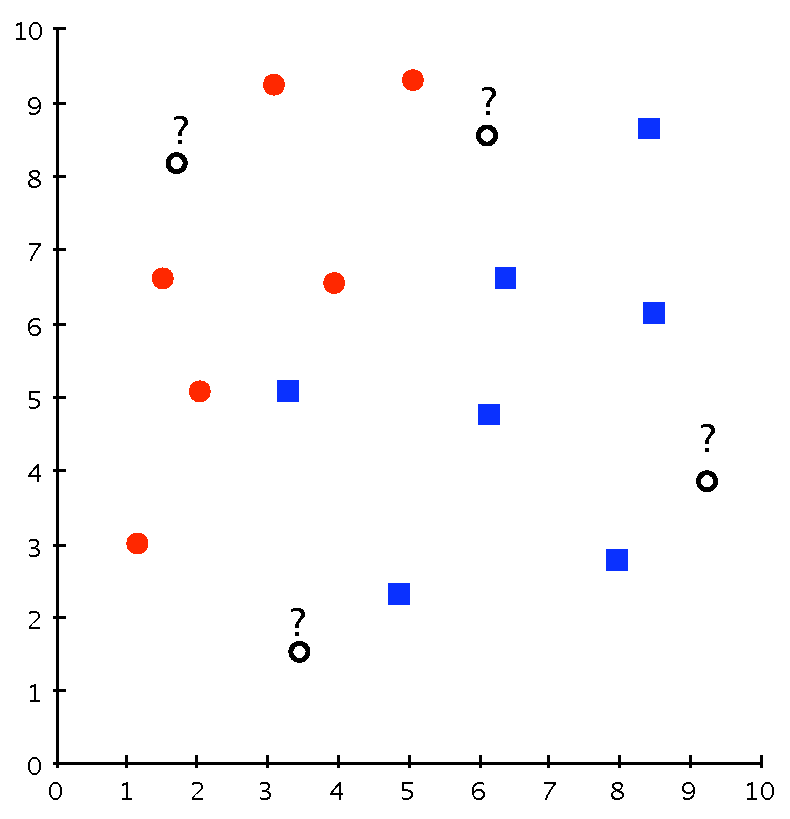
\includegraphics[height = 5.5cm]{classification} \> 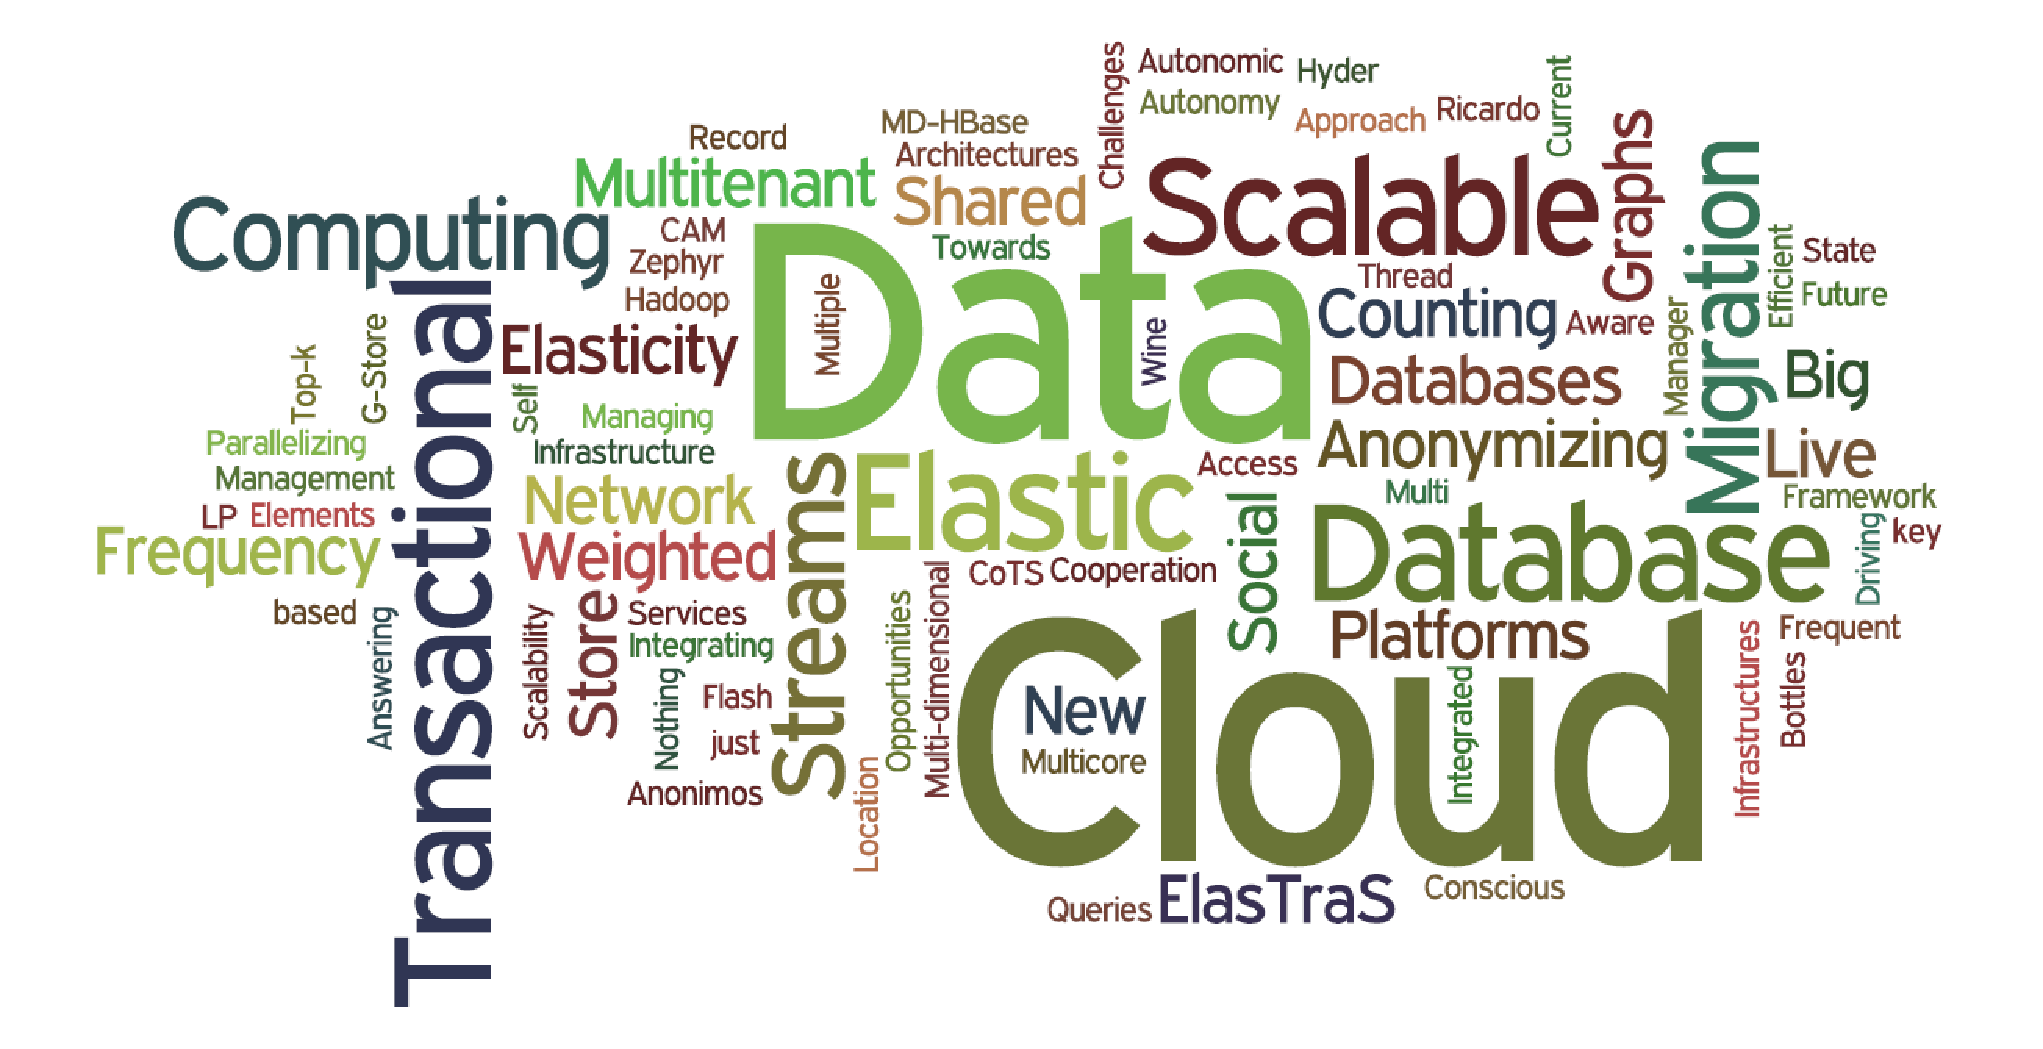
\includegraphics[width = 9cm]{word-cloud}\\  \vspace*{1cm} \\
   \>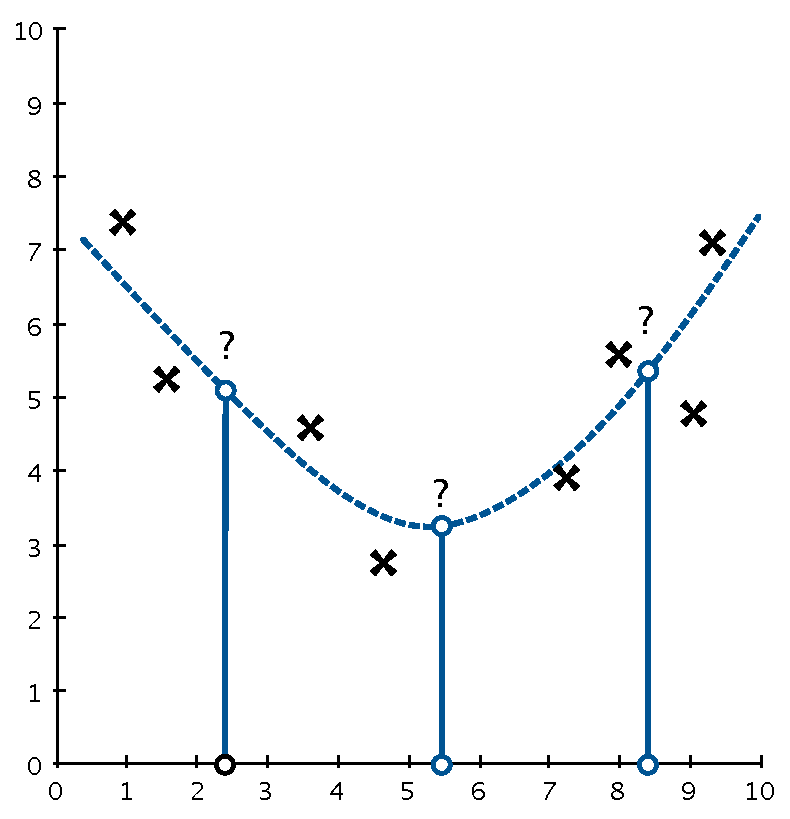
\includegraphics[height = 5.5cm]{regression}   \>  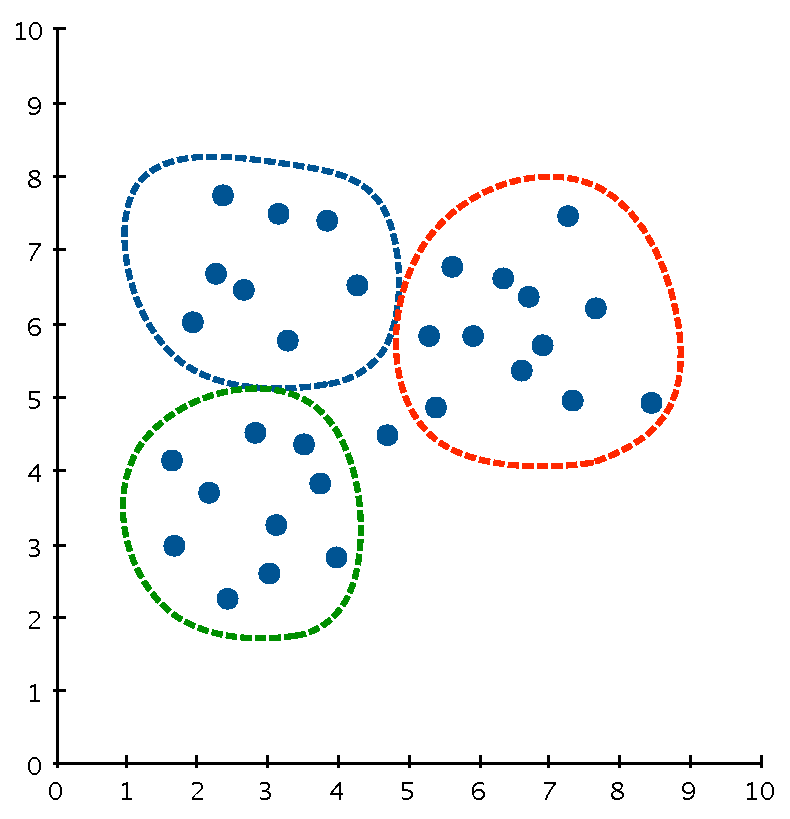
\includegraphics[height =5.5cm]{clustering}\\
\end{tabbing}

\foilhead[-1cm]{Four basic issues you have to solve}

\enlargethispage{3cm}
\begin{tabbing}
 \hspace*{2cm}\=\hspace*{10cm}\=\kill
   \> 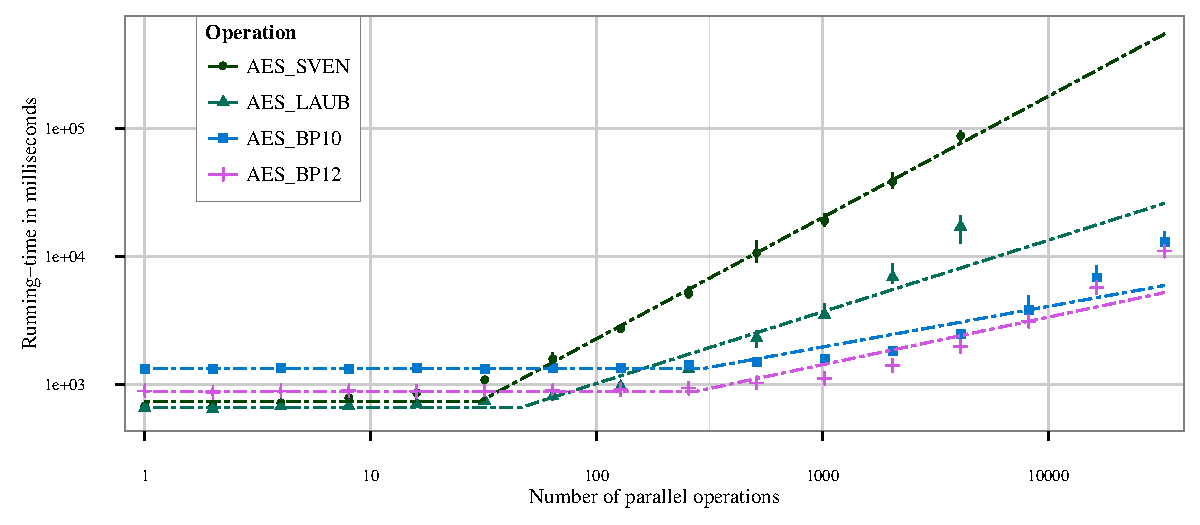
\includegraphics[height = 5.5cm, trim=2.5cm 0cm 3.8cm 0cm, clip]{aes-full-time}
   \> 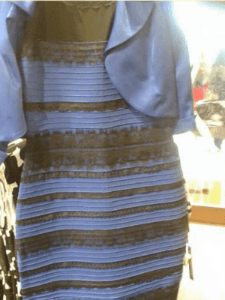
\includegraphics[height = 5.5cm, trim=0cm 0cm 0cm 0cm, clip]{the-dress}
\hspace*{0.15cm}
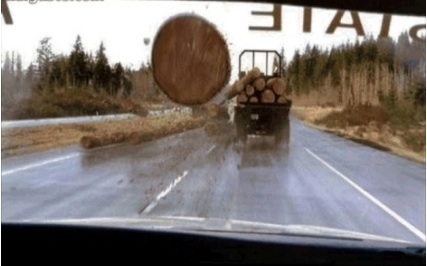
\includegraphics[height = 5.5cm, trim=4cm 0cm 4cm 0cm, clip]{logs-falling}\\

   \> 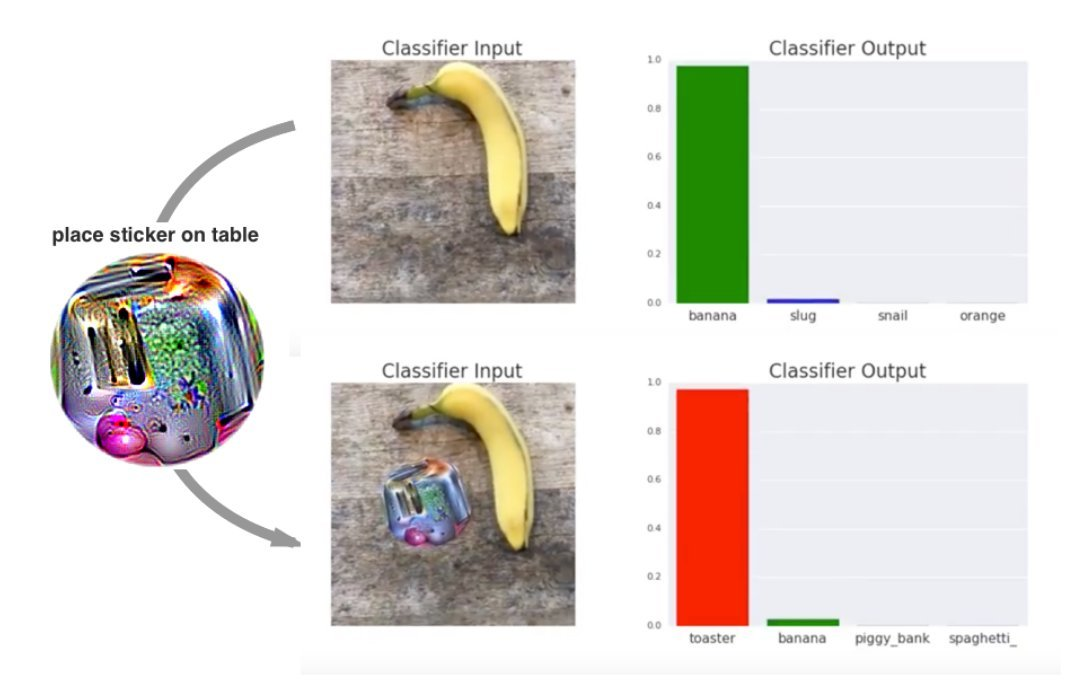
\includegraphics[height = 5.5cm]{adversarial-learning}
   \> 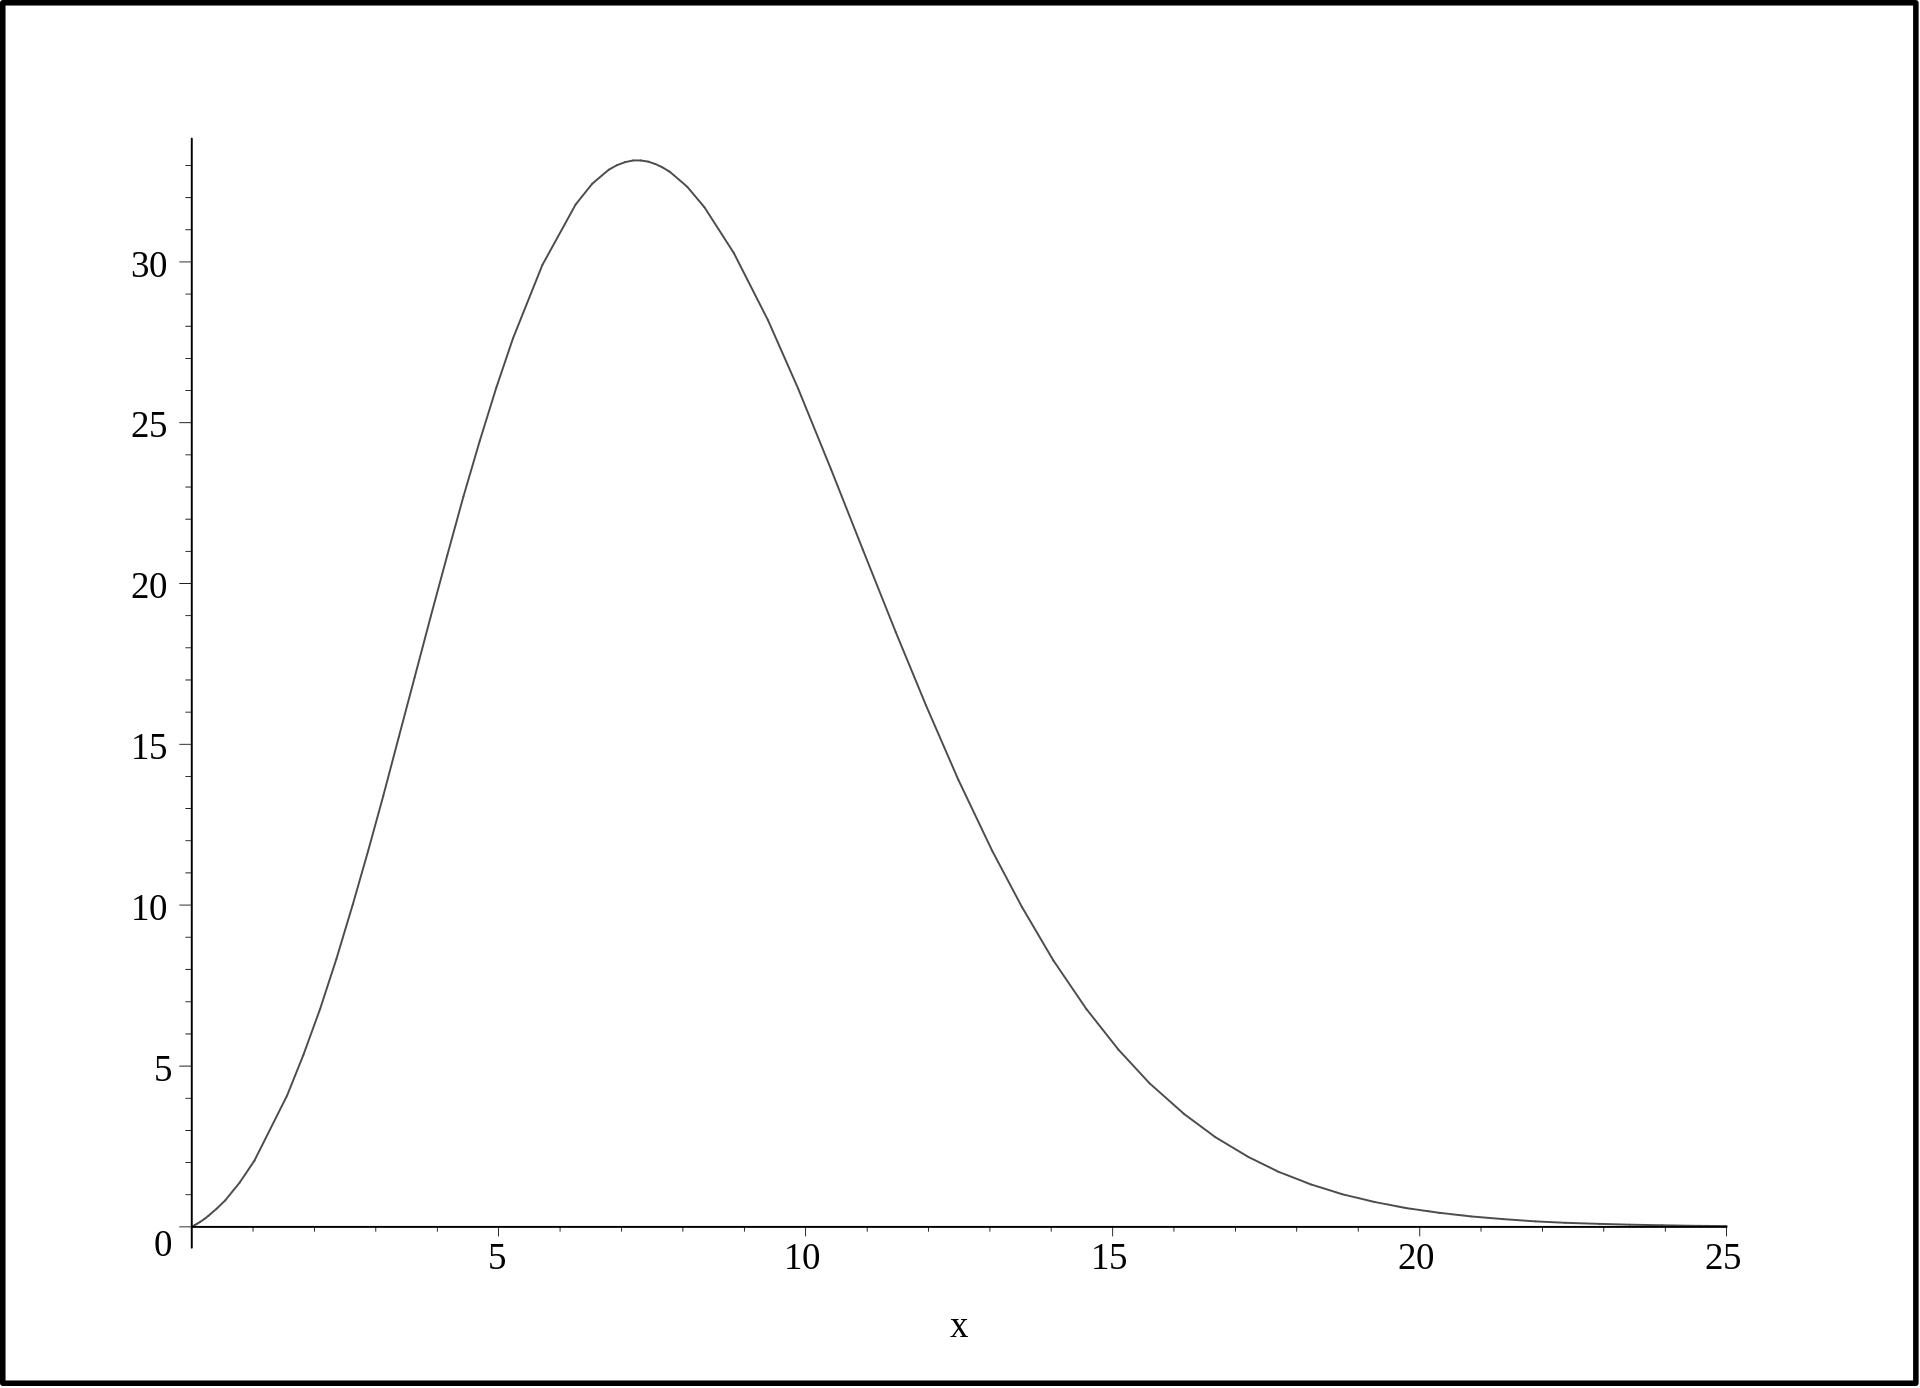
\includegraphics[height = 5.5cm, trim=-4.5cm 0cm -4.5cm 0cm, clip]{curse-of-dimensions}
\end{tabbing}




%\frame{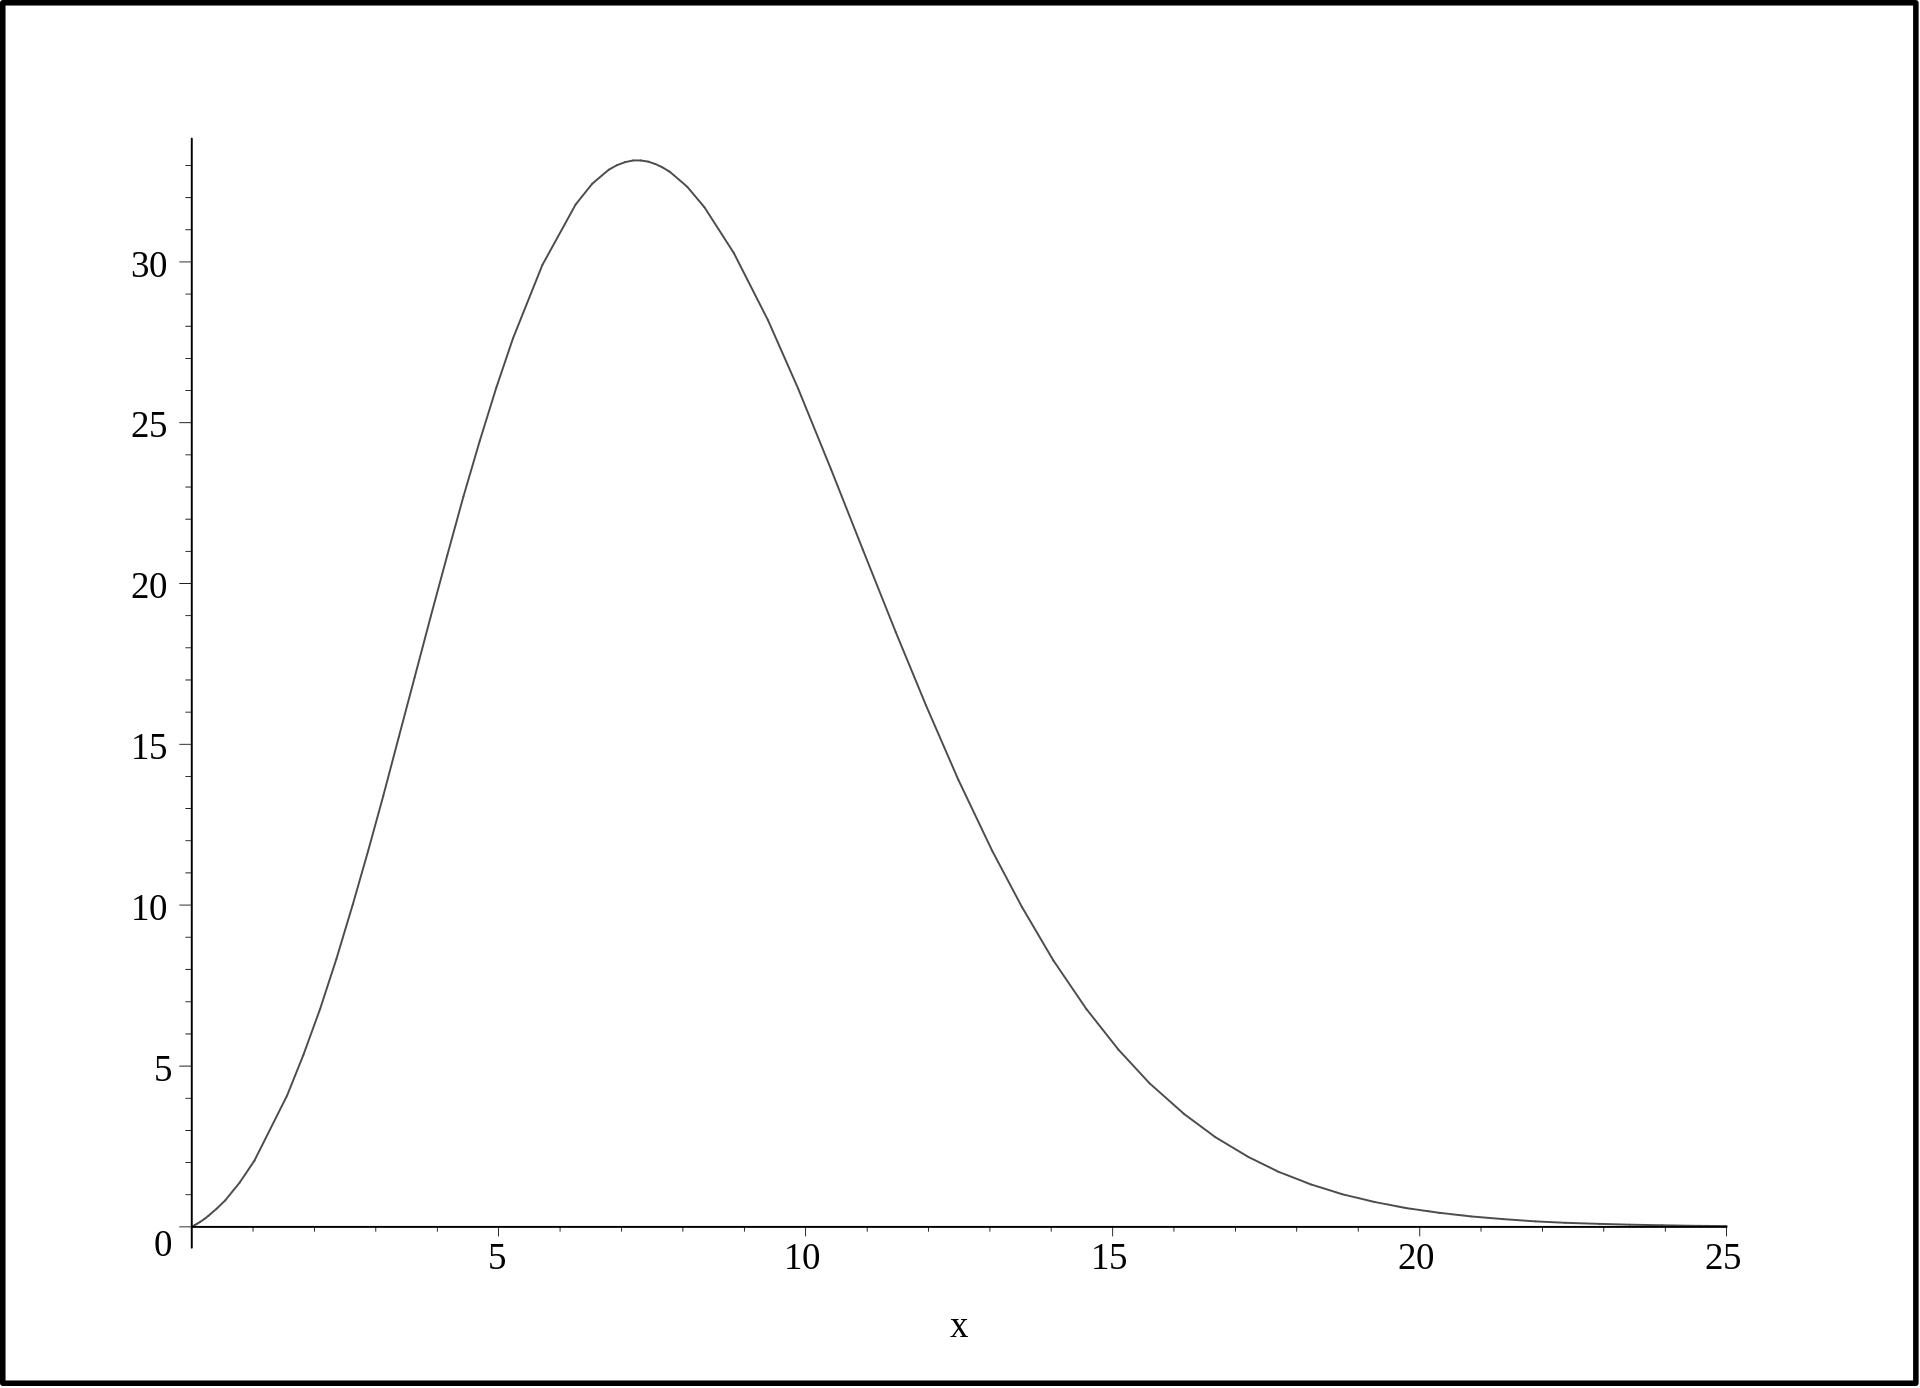
\includegraphics[height = 5.5cm, trim=-4.5cm 0cm -4.5cm 0cm, clip]{curse-of-dimensions}}

\foilhead[-1cm]{Main inference prodedure}

\illustration[height=9cm]{main-procedure}

Usually no machine learning method works on real data without tweaking 
\begin{triangles}
 \item The signal might be missing form the data 
 \item The method uses wrong features for its predictions 
\end{triangles}


\foilhead[-1cm]{Features are more important than method}

\illustration[width=10cm]{checker-board}

The signal is completely lost if we observe a single feature: $x$-coordinate or $y$-coordinate. By knowing both features the pattern is clearly visible.



\foilhead[-1cm]{Do not learn what you already know!}
\illustration[scale=0.8]{physical-modelling}

Sometimes we know the overall structure of the model
\begin{triangles}
 \item In robotics the effect of actuators can be expressed directly
 \item Sometimes we know some governing rules form previous studies
\end{triangles} 
In such cases, learning the entire model with machine learning is wasteful
\begin{triangles}
 \item Locate the parts of the model that are undefined
 \item Use machine learning to find missing links 
\end{triangles} 

\end{document}



\foilhead[-1cm]{Rule-based prediction}
\illustration[scale=0.8]{rule-inference}

\textbf{Task.} Given a set of examples find a set of rules such that these rules
\begin{triangles}
\item cover most of the examples
\item make as few error as possible on the training set
\end{triangles}\bigskip

\textbf{Important notions and metrics:}
\begin{triangles}
\item cover, support, confidence, lift, mutual information, $\ldots$   
\end{triangles}\medskip

\foilhead[-1cm]{Support and confidence}
\illustration[scale=0.7]{support-and-confidence}


Let $\alpha$ denote the rule   $x_1=a_1\wedge\cdots\wedge x_k=a_k\Rightarrow y=b$. Then
\begin{triangles}
\item The support of a rule $\supp(\alpha)$ is the fraction of samples for which the condition $x_1=a_1\wedge\cdots\wedge x_k=a_k\wedge y=b$ holds.

\item Confidence of a rule $\alpha$ is the fraction of correct predictions:
\begin{align*} 
\conf(\alpha)=\frac{\#\set{example:x_1=a_1\wedge\cdots\wedge x_k=a_k\wedge y=b}}{\#\set{example:x_1=a_1\wedge\cdots\wedge x_k=a_k}}
\end{align*} 
\end{triangles}

\foilhead[-1cm]{Precision and recall}

\enlargethispage{1cm}
\illustration[scale=0.75]{precision-and-recall}

Utility of any rule can be quantified in terms of precision and recall:
\begin{align*}
\precision&=\frac{\#\textsc{True Positives}}{\#\textsc{Positive Predictions}}=\frac{\textsc{TP}}{\textsc{TP}+ \textsc{FP}}\\
\recall&=\frac{\#\textsc{True Positives}}{\#\textsc{Positive Labels}}=\frac{\textsc{TP}}{\textsc{TP}+ \textsc{FN}}
\end{align*}
Precision and recall depend on the dataset which is used to test the rule.



\foilhead[-1cm]{Why rule-based prediction does not work?}

\illustration[width=23cm]{rule-coverage}

Only few rules are frequent enough to be captured by gathered examples.
 
\foilhead[-1cm]{What is a decision tree?}

Decision tree is a systematic way to split the feature space into rectangular blocks. Each block get a single putative label by majority voting.  

There are many decision tree learning algorithms:
\begin{triangles}
\item ID3, C4.5, C5, $\ldots$
\end{triangles}

They all share the same divide and conquer strategy, which recursively divides data into subsets until homogenous regions are discovered. 

The difference is in the details:
\begin{triangles}
 \item Which features are used for splitting?
 \item What is the criterion for choosing the best split? 
 \item What is the criterion for stoping?
 \item Do we prune overly complex rules?
 \item How the decision is made in leaf nodes? 
\end{triangles}  

\foilhead[-1cm]{Basic ideas through an example}

\includegraphics[height = 12cm]{decision-tree-1}% 
\vspace*{-11cm}\\ \hspace*{12cm} 
\begin{minipage}[c]{12cm}
Lets split the data based on $X_1$
\begin{triangles}
 \item $X_1=R$
 \item $X_1\in\set{G,B,W}$ \vspace*{2ex}
\end{triangles}
and study the first part $\ldots$
\end{minipage} \\

\foilhead[-1cm]{Basic ideas through an example}

\includegraphics[height = 12cm]{decision-tree-2}% 
\vspace*{-11cm}\\ \hspace*{12cm} 
\begin{minipage}[c]{12cm}
This part can be split based on $X_2$
\begin{triangles}
 \item $X_2=E$
 \item $X_2\in\set{B,A,G}$ \vspace*{2ex}
\end{triangles}
Lets study the second part $\ldots$
\end{minipage} \\


\foilhead[-1cm]{Basic ideas through an example}

\includegraphics[height = 12cm]{decision-tree-3}% 
\vspace*{-11cm}\\ \hspace*{12cm} 
\begin{minipage}[c]{12cm}
This part can be split based on $X_2$
\begin{triangles}
 \item $X_2\in\set{G,E}$
 \item $X_2\in\set{B,A}$ \vspace*{2ex}
\end{triangles}
But the cut is not clean $\ldots$
\end{minipage} \\


\foilhead[-1cm]{Basic ideas through an example}

\includegraphics[height = 12cm]{decision-tree-4}% 
\vspace*{-11cm}\\ \hspace*{12cm} 
\begin{minipage}[c]{12cm}
The lower half is homogenous enough!
\end{minipage} \\



\foilhead[-1cm]{Final result}

\includegraphics[height = 12cm]{decision-tree-6}% 
\vspace*{-11cm}\\ \hspace*{12cm} 
\begin{minipage}[c]{12cm}
\begin{triangles}
 \item If $X_1\in\set{R}$
   \begin{ddiamonds}
    \item If $X_2\in\set{B, A, G}$ then $\ldots$ 
    \item Else $X_2\in\set{E}$ then $\ldots$ 
   \end{ddiamonds}
 \item $X_1\in\set{B,G,W}$ 
    \begin{ddiamonds}
    \item If $X_2\in\set{B, A}$ then $\ldots$ 
    \item Else $X_2\in\set{G, E}$ then\vspace*{0.5ex} 
    \begin{darrows}
     \item If $X_1\in\set{B,G}$ then $\ldots$
     \item Else $X_1\in\set{E}$ then $\ldots$ 
    \end{darrows}
   \end{ddiamonds}
\end{triangles}
\end{minipage} \\


\foilhead[-1cm]{Which attribute to choose for splitting?}

It makes sense to split the data so that resulting parts are more homogenous.
ID3 algorithm uses entropy and entropy gain to choose the split


\textbf{Frequency.} We can compute probability for each value of the target $Y$: 
\begin{align*}
\pr{Y=a}=\frac{\#\set{examples: Y=a}}{\#\set{examples}}
\end{align*}
\textbf{Entropy.} We can express the overall entropy in bits
\begin{align*}
H(Y)=-\sum_{a\in Dom(Y)}\pr{Y=a}\cdot\log_2(\pr{Y=a})
\end{align*}

\foilhead[-1cm]{Which attribute to choose for splitting?}

It makes sense to split the data so that resulting parts are more homogenous.
ID3 algorithm uses entropy and entropy gain to choose the split


\textbf{Entropy gain.} Assume that the dataset $S$ is split into disjoint sets $S_1,\ldots, S_k$. Then the corresponding entropy gain is 
\begin{align*}
\mathrm{Gain}= H_S(Y)-\sum_{i=1}^k\frac{\abs{S_i}}{\abs{S}}\cdot H_{S_i}(Y)
\end{align*}
where $H_S(Y)$ denotes the entropy commuted over $S$ and $H_{S_i}(Y)$ denotes the entropy computed over $S_i$. The entropy gain measures how much the split makes the target value distribution more homogenous.


\foilhead[-1cm]{How to split the data according the  attribute?}

\begin{triangles}
\item The answer is obvious for binary attributes. 
\item For categorical attributes the data is according to individual values
\item For continuous attributes the data is usually split according to a threshold value $t$. The value $t$ itself is chosen to maximise the information gain. 
\end{triangles}


\foilhead[-1cm]{When is it right time to stop?}

Recursive splitting lead us quickly to datasets which consists of few samples. These datasets are not informative any more:
\begin{triangles}
\item labelling errors, measurement errors, missing examples, $\ldots$  
\end{triangles}\bigskip\bigskip

There are many alternative strategies to detect 
\begin{triangles}
\item Early stopping based on dataset size
\item Early stopping based on statistical tests
\item Early stopping using holdout data
\item Bottom-up pruning strategy
\item Rules and rule generalisation
\item Rule prioritisation 
\end{triangles}



\foilhead[-1cm]{Rule prioritization}

\textbf{Pruning}
\begin{triangles}
\item Convert all leaf-node decisions into rules
\item For each rule drop assumptions that decrease precision on validation set 
\item Sort rules by estimated confidence
\end{triangles}\vspace*{1cm}

\textbf{Prediction}
\begin{triangles}
\item Choose the rule with highest confidence among applicable rules. 
\end{triangles}\vspace*{1cm}
 

\textbf{Corollary.} Decision-tree learning is a systematised way to learn rules:
\begin{triangles}
\item Discovered rules cover the entire feature space. 
\item Recursive splitting assures that rules have orthogonal assumptions. 

\end{triangles}\vspace*{1cm}


\foilhead[-1cm]{Why does decision-tree learning work?}

\textbf{Under iid assumption.} All samples are generated by the same procedure. Previously generated examples do not influence future examples.  

\textbf{What can we hope for?}
\begin{triangles}
\item The decision tree might not be able to capture the true solution. 
\item We can only hope that the learning algorithm provides the best tree. 
\item Even that is impossible for all examples. Only probabilistic guarantees. 
\end{triangles}\vspace*{1cm}

\textbf{Guarantees form statistics}
\begin{triangles}
\item Given enough data the tree structure stabilises if tree size is bounded
\item Given enough data the majority voting in the leaf nodes is optimal  
\item Hypothesis space is complete 
\end{triangles}


\end{document}

